\subsection*{Hold}
\addcontentsline{toc}{subsection}{Hold}

\textbf{Задание:}\\
Реализовать модель СМО с применением блока Hold.\\

\textbf{Решение:}\\
При моделировании СМО можно столкнуться с ситуацией, когда количество агентов, поступающих в очередь превышает вместимость этой очереди. Для того, чтобы не потерять этих агентов, не создавая дополнительный блок \textit{Delay}, можно осуществлять задержку агентов с помощью блока \textit{Hold}.\\

Блок \textit{Hold} блокирует/снимает блокировку с потока агентов на определенном участке блок-схемы. Он используется, например, когда блок может принимать агентов, но вы не хотите (временно) продолжать их обработку или когда нужно заблокировать поступление агентов только от какого-то определенного блока, в то же время принимая агентов, приходящих с выходных портов других блоков.\\

Рассмотрим СМО, состоящую из источника, очереди, блока задержки и стока, в которую добавим блок Hold. (Рисунок \ref{fig:hold_anylogic})
\begin{figure}[h]
	\centering 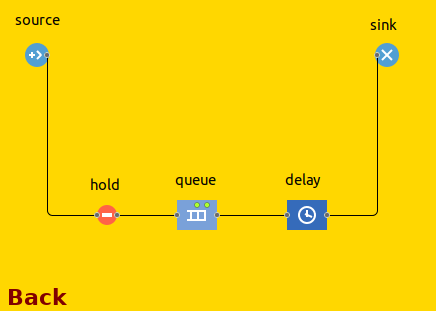
\includegraphics[scale=0.34]{hold_anylogic}
	\caption{Схема СМО с блоком \textit{Hold}}
	\label{fig:hold_anylogic}
\end{figure}

Логика блокировки и снятия блокировки потока агентов реализована в блоке \textit{Queue}. (Рисунок \ref{fig:hold_anylogic2})
\begin{figure}[h]
	\centering 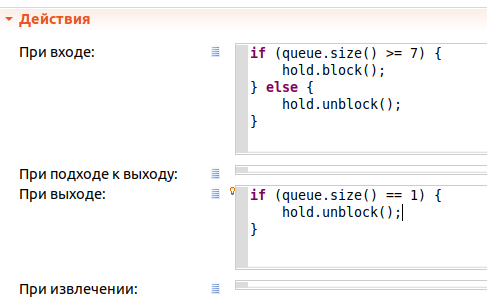
\includegraphics[scale=0.36]{hold_anylogic2}
	\caption{Логика работы с блоком \textit{Hold}}
	\label{fig:hold_anylogic2}
\end{figure}

\newpage

При входе проверяем достигнута ли максимально возможная вместимость, в данном случае 7, если да, то осуществляется блокировка. В случае, когда размер очереди становится равен 0, то блокировка с агентов снимается.\\

Таким образом, была рассмотрена СМО, в которой осуществляется блокировка поступления агентов в очередь.